\section{Implementation Details}
    \subsection{Facial Landmarks Tracking and normalizing}
        The first step of this authentication system is to track the facial landmarks from the video footage. We achieve this by employing an open source facial tracking algorithm called SeetaFace~\cite{SeetaFace-toolbox-web}. This algorithm can real-time detect human face and tracks the facial landmarks based on deep convolutional neural network (CNN)~\cite{Krizhevsky2012ImageNet}. For each video frame, the algorithm tries to localize the position of the facial landmarks.
        \subsubsection{Track Facial Landmarks}
            The SeetaFace algorithm automatically detects and tracks face landmarks based on the deep CNN model trained offline. For each video frame, the algorithm first detects the face using scan window mechanism. The size of scan window has an prominent effect on real-time detection speed. We set the window size to no less than $50$ which is found to give good tradeoff between the detection speed and accuracy in our initial design experiment using $35$ expression videos\footnote{To provide a fair evaluation, the video footages used in all our initial test runs in the design phase are different from the ones used later in evaluation}. SeetaFace has three modules: (1) face detection module that follows the face across consecutive frames under the assumption that the frame-to-frame facial expressions are visible; (2) face alignment module that tracks the facial landmarks and localize its position on the face based on the face area detected in (1); and (3) face identification module that is applied to recognize human's identify by simply calculating the cosine similarity of two facial images. It is worthwhile to mention that our system just employs the first two modules which is enough for our system to get the position of facial landmarks.

            The SeetaFace face detection module is constructed by using Funnel-Structured (\emph{FuSt}) cascade scheme. The \emph{FuSt} cascade scheme consists of coarse-to-fine cascade classifiers: multiple view-specific fast LAB  cascade for coarse face selection at the top stage, followed by the coarse Multilayer Perceptron (\emph{MLP}) cascade for facial candidate windows verification at the middle stage and a fine \emph{MLP} cascade for localize the face position at the bottom stage~\cite{Wu2016Funnel}. In the following frames, the detection module detects the face based on a model trained in advance with approximately $200K$ labeled face images by using the above three coarse-to-fine cascade classifiers. For each video frame, the face module detects the potential face areas according to the sliding window paradigm and finally yields the face area by going through the cascade classifiers stage by stage. Taking the detected face area as an input, the face alignment module localize the facial landmarks by exploiting a Coarse-to-Fine Auto-encoder Networks (\emph{CFAN})~\cite{Zhang2014Coarse}. The \emph{CFAN} is comprised of a few successive Stacked Auto-encoder Network (\emph{SANs}). The first \emph{SAN} aims to predicts the approximate facial landmark locations based on the detected face area and then the following \emph{SANs} progressively refine the landmark locations by the joint local features extracted around the current landmarks. Finally, the five facial landmarks locations will be stored for further feature extraction. Detail discussion of SeetaFace can be found at~\cite{SeetaFace-toolbox-web}. Sometimes the algorithm may fail to detect the face in some video frames due to drastically head pose. If this happen, our algorithm will tolerate a certain degree of detection failure but it will ask the user re-authenticate if many detection failure (more than 30\%) occurs.

        \begin{figure}
            \centering
            \subfigure{
                \begin{minipage}[t]{0.19\textwidth}
                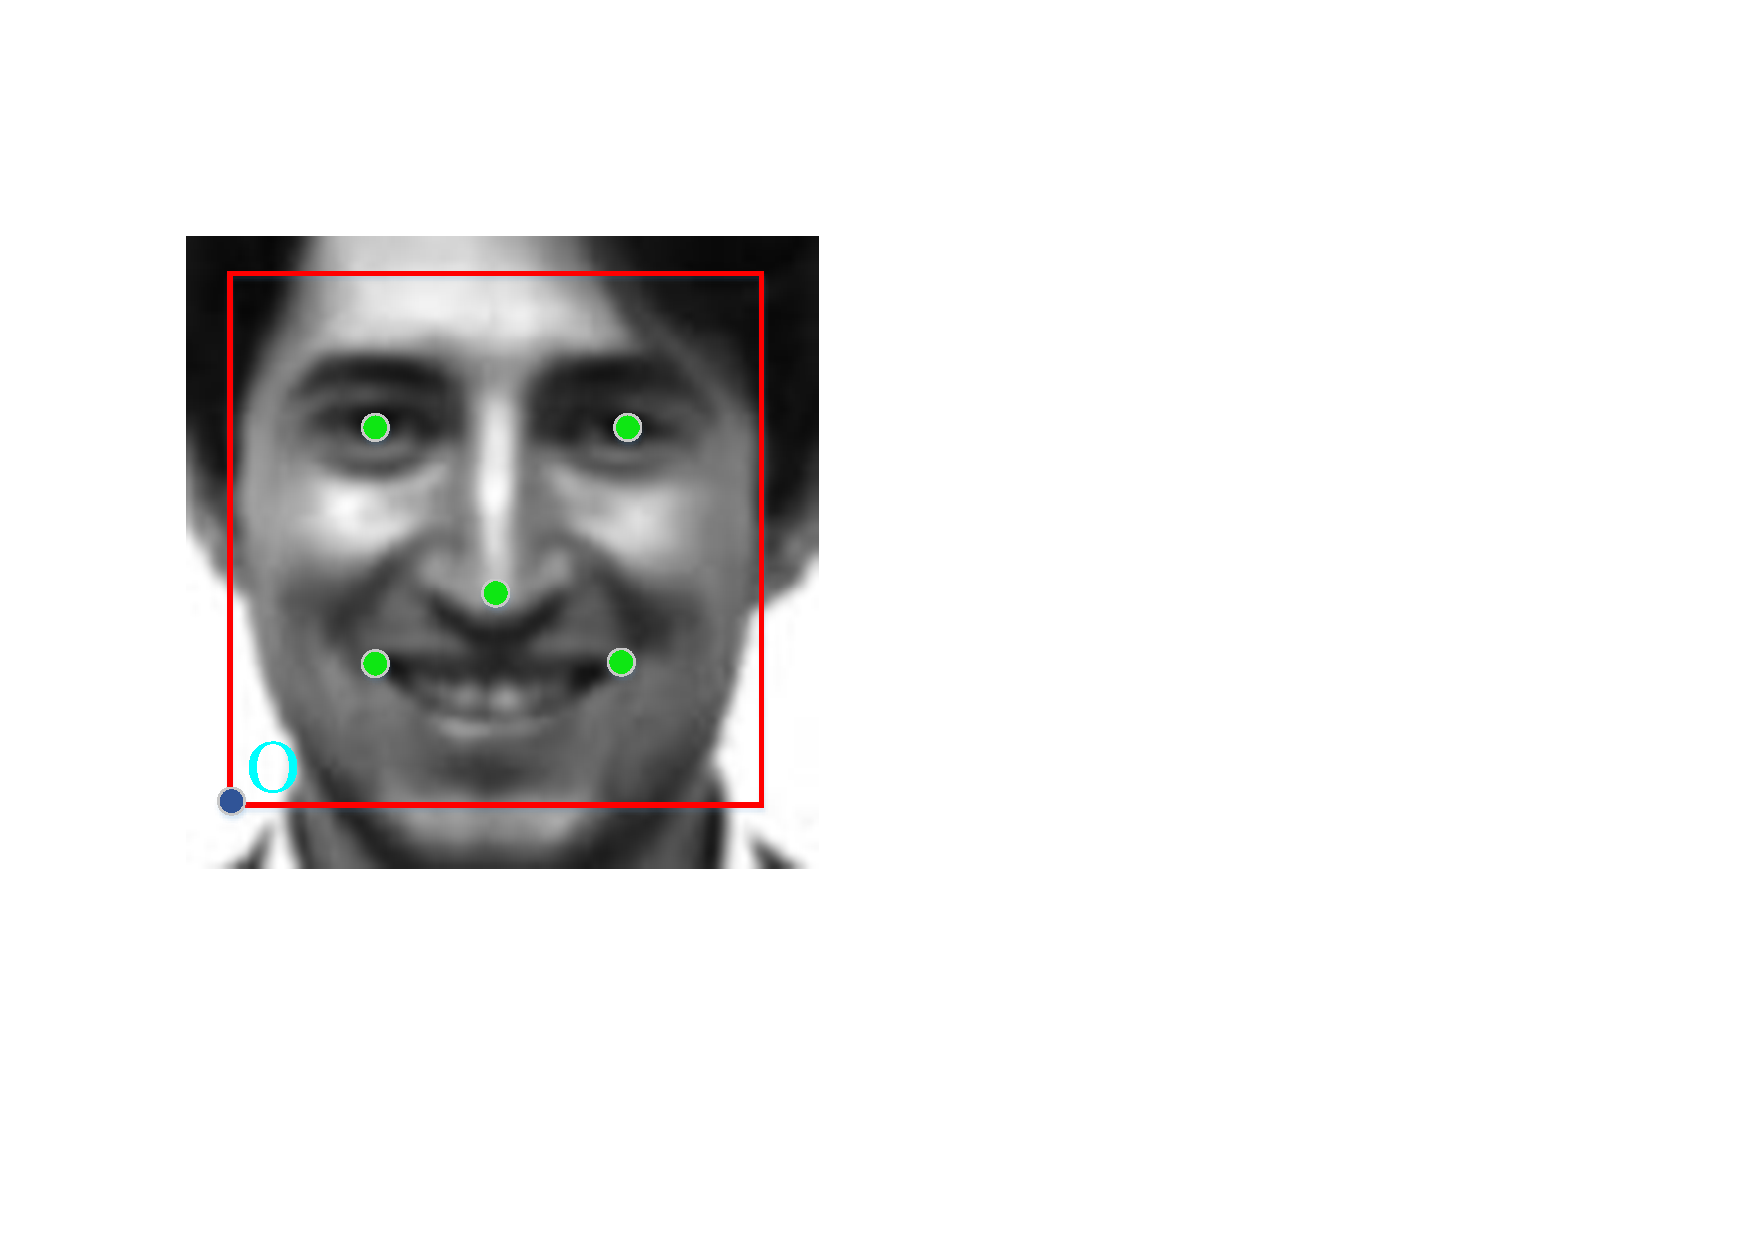
\includegraphics[width=0.8\textwidth]{fig/normalization1.pdf}\\
                \centering \footnotesize (a) a frontal-view face
                %\FIXME{Need to mark the starting point and turning point}
                \end{minipage}
            }
            \hspace{0.25cm}
            \subfigure{
                \begin{minipage}[t]{0.19\textwidth}
                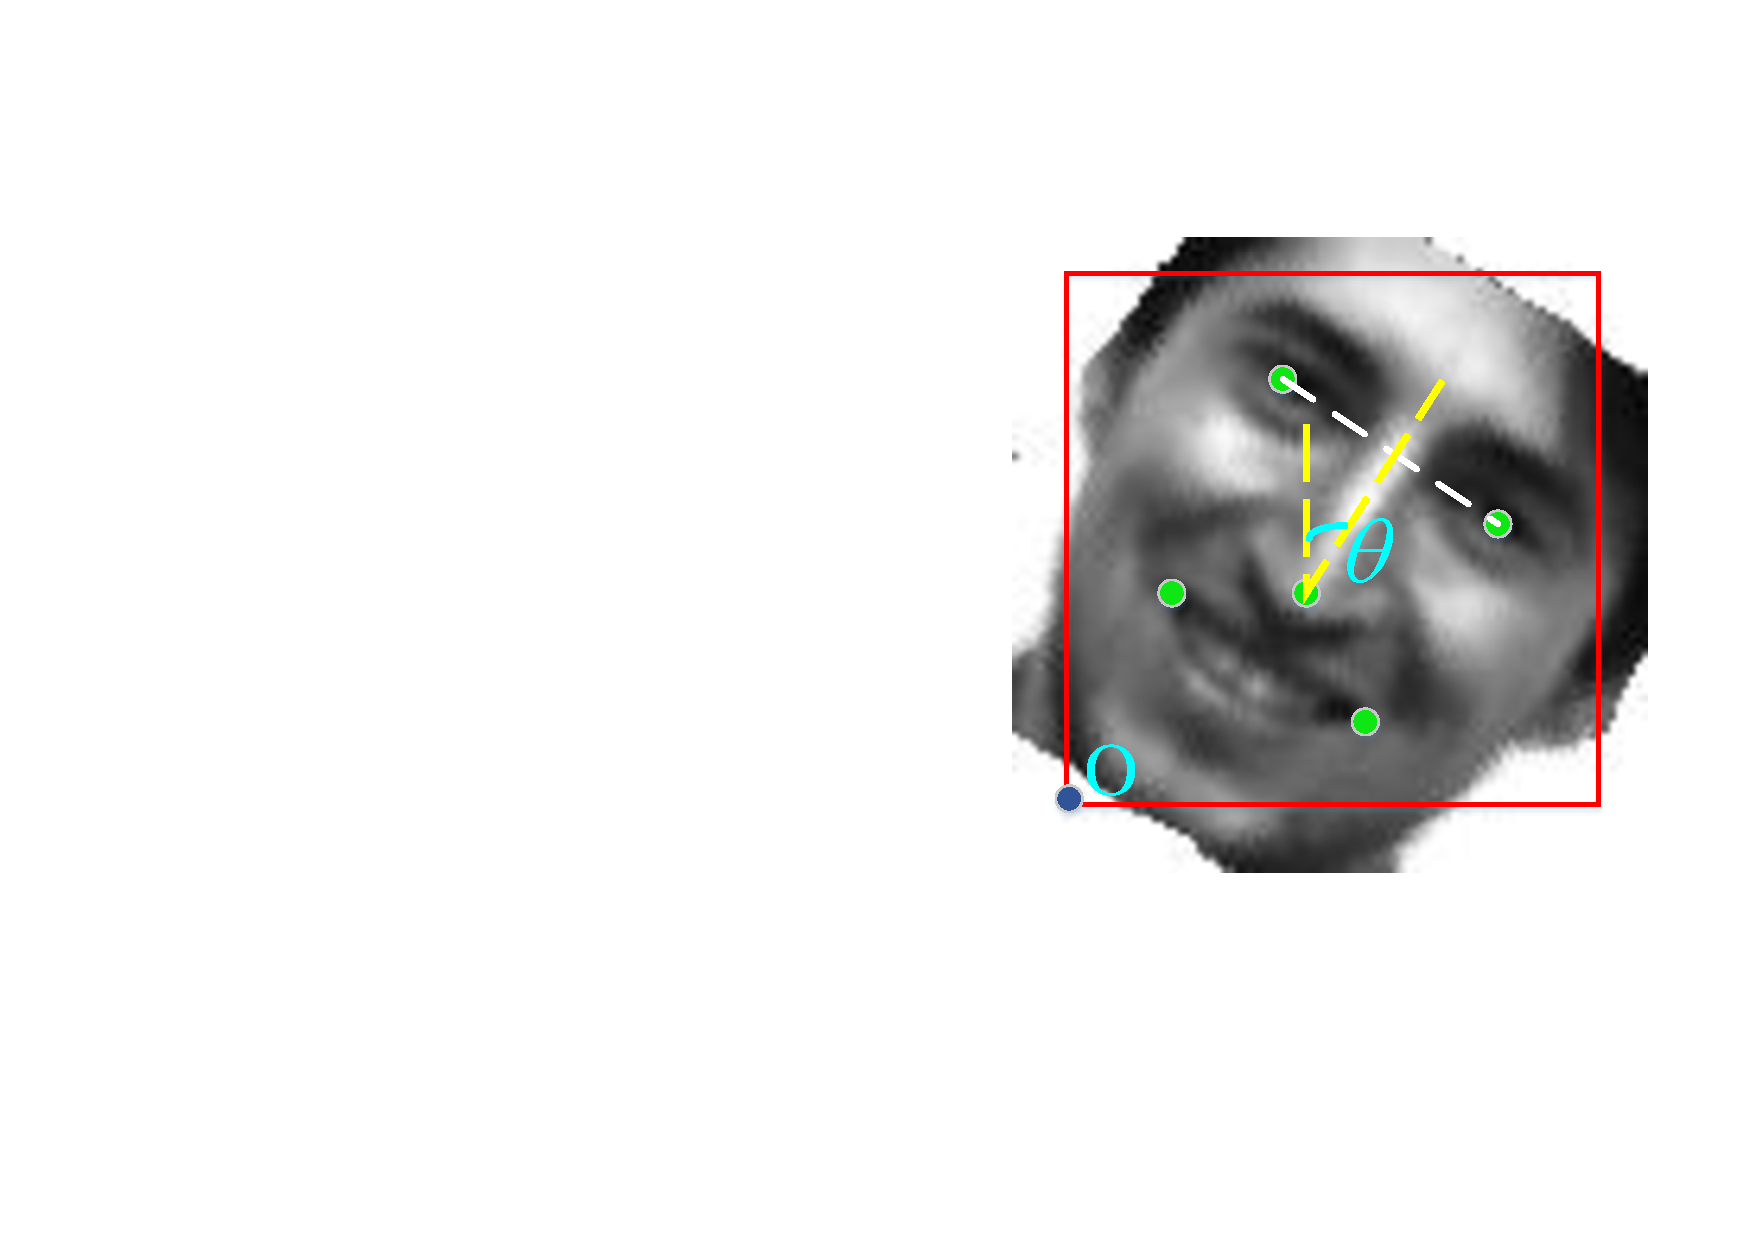
\includegraphics[width=0.8\textwidth]{fig/normalization2.pdf}\\
                \centering \footnotesize (b) a camera's view face
                \end{minipage}
            }
            \caption{Facial expressions and landmarks under two different view angles. The rotation angle, $\theta$, is the angle between the midperpendicular of connection of two eye landmarks and a vertical line.}
            \label{fig:normalization}
        \end{figure}
        
        \begin{algorithm}[!t]
            \centering
            \caption{Face Normalization Algorithm}
            \small
            \label{alg:normalization}
            \begin{algorithmic}[1]
                \REQUIRE~~\\
                    $EV$: Expression Video  \\
                    $angleThreshold$: The threshold of rotation angle\\
                    $fixedSize$: The fixed size of uniform facial images\\
                    %$locationTh$: Threshold of fingertip location changes\\
                \ENSURE~~\\
                    %$<$start,end$>$: Start and end of the unlocking video segment \\
                    $NF[]$: Normalized facial expression images under frontal view\\
                \STATE $flag \leftarrow openFrontFacingCamera()$
                \WHILE{$flag$}
                    \STATE $eF \leftarrow captureExpressionFrames()$ \\
                    \IF{$!ef$}
                        \STATE $fL[] \leftarrow getFacialLandmarks(eF)$ \\
                        \STATE $rA \leftarrow calculateRotationAngle(fL[])$
                        \IF{$rA>angleThreshold$}
                            \STATE $fI \leftarrow rotateFacialFrame(eF,rA)$
                        \ELSE
                            \STATE $fI \leftarrow eF$
                        \ENDIF
                        \STATE $NF[] \leftarrow zoomFacialImage(fI,fixedSize)$
                    \ENDIF
                \ENDWHILE
            \end{algorithmic}
        \end{algorithm}
        \subsubsection{Face Normalization}
            By default, The face alignment algorithm reports the facial landmarks positions with respect to the bottom-left pixel of the face shown as Figure~\ref{fig:normalization} (a) point $O$. However, the size of face detected by face detection module are uniform under different usage scenarios as the distance between the face and the phone camera are not the same according to individual's habits. For example, this distance when one lies in bed is typically shorter than the one when he stands or sits. Furthermore, the head pose still results in the rotation of the face in specific situation such as playing the smartphone in bed. Those can drastically affect the value of the dynamic facial features, leading to misidentification of users in authentication phase.

            Our approach to solve the above challenges can be divided into two steps. The first step is to rotate the face from the camera's view to the frontal view. To do so, we need to evaluate the rotation angle of the face. If the value of rotation angle is more than a threshold, this approach will automatically rotate the face to the frontal side. The rotation angle can be figured out according to the part of the facial landmarks including the left and right center of the eyes and the nose tip. This is illustrated in Figure~\ref{fig:normalization} (b). Based on the estimated filming angle, $\theta$, we use the following formula to transform the face from the camera's view to the frontal view:
            \begin{equation}
                P=TP^{'} \qquad, \qquad  T=\left[ \begin{matrix} \cos\theta & -\sin\theta \\ \sin\theta & \cos\theta \end{matrix} \right]
            \end{equation}

            where $T$ is a Transformation Matrix, $P^{'}$ is the coordinate of a point of the face, and $P$ is the resulting coordinate after the transformation. For each video frame, our algorithm individually calculates the rotate angle and perform the transformation, because the rotation angle may change across video frames.

            The second step is to normalize the facial size. To uniform the face size, we map the face detected by face detection module to a fixed size which is $200\times200$ pixels. To do so, our algorithm uses the bilinear interpolation algorithm~\cite{Gribbon2004A} to zoom in/out the current face comparing to the fixed size.

            The algorithm for face normalization process is described in Algorithm~\ref{alg:normalization}. The input to the algorithm is the facial expression video footage and the threshold of rotation angle, and the output of the algorithm is the frontal facial images. To normalize the facial expression images, we first figure out the rotation angle. To do so, the coordinates of the five facial landmarks are tracked (line 5), and the rotation angle can be calculated according to the angle between the vertical ling and the midperpendicular of connection line of two eyes landmarks (line 6). IF the rotation angle is more than a threshold, $angleThreshold$, the facial expression image will be rotated to frontal view and zoomed in/out to the fixed size (lines 8 and 12).  Specifically, the angle threshold, $angleThreshold$, is set to 5 and the fixed size of facial images, $fixedSize$ is set to $200\times200$ pixels. To determine the thresholds, we have evaluated a range of possible values in our initial design experiments to chose the best performing values.

    \subsection{Replay Detection}
        
    \subsection{Feature Extraction}

    \subsection{Identity Authentication}

